\section{Architecture}
The following section provides an insight over the structure and architecture
of the application.
\subsection{Components}
The components presented in the Figure \ref{componentDiagram} are divided into
two categories:
\begin{description}
  \item[yellow] already existing components
  \item[white]  components, which have to be implemented.
\end{description}
SQL Lite database was chosen, because it is directly supported by the Android
SDK. The same reasoning applies to the selection of the Google Maps API.
 \begin{figure}[h]
  \caption{LocationManager Component Diagram}
  \label{componentDiagram}
  \center
  	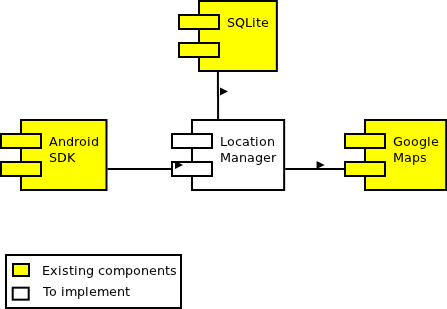
\includegraphics[scale=0.75]{../resources/ComponentDiagram.png}
\end{figure}

 \begin{figure}[h!]
  \caption{LocationManager Class Diagram}
  \center
  	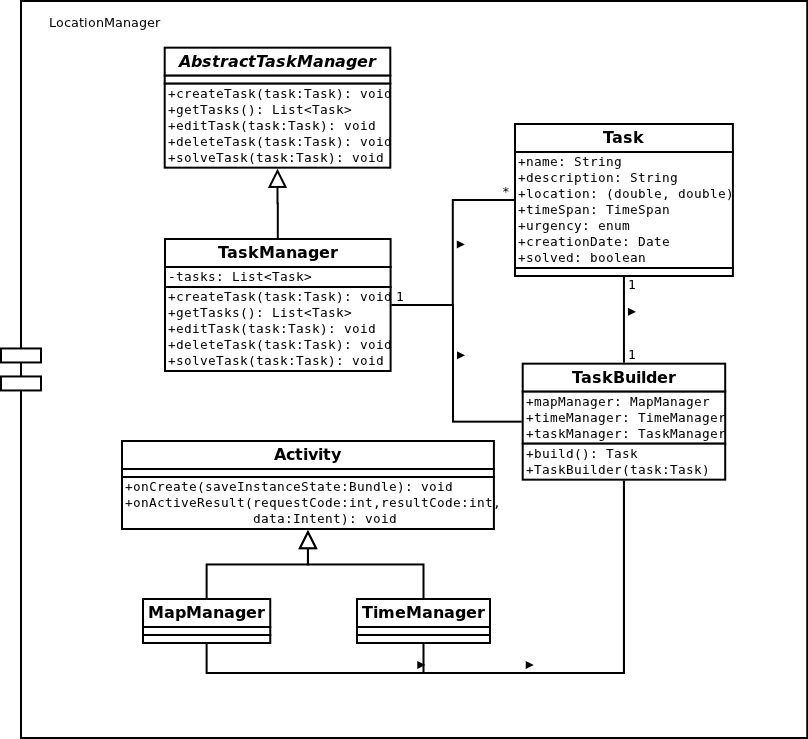
\includegraphics[scale=0.5]{../resources/ClassDiagram.png}
\end{figure}
The \emph{TaskManager} is the core component of the application. It takes care
of creating, editing, saving and deleting tasks. The \emph{TaskBuilder} is the
central component of the delivery system of the application. It controls the
\emph{MapManager}, the \emph{TimeManager} and the \emph{TaskManager}
respectively. Both the \emph{MapManager} and the \emph{TimeManager} are derived
from the \emph{Activity}, which is the main part of the Android application
life-cycle. The \emph{MapManager} handles the view of the map, by using the
Google Maps API. The \emph{TimeManager} uses standard Android widgets to assist
the user in selecting the time span.
\newpage
\subsection{Used Technologies}
The application is written in Java and built with Eclipse. The SQL Lite database
was used to persist the tasks and further vital information. Android API were
used to determine the current location. The Google Maps API was used to visually
represent the coordinates.